\section{Flag 04 - Cookies}

\paragraph{df2eb4ba34ed059a1e3e89ff4dfc13445f104a1a52295214def1c4fb1693a5c3}
\begin{center}
    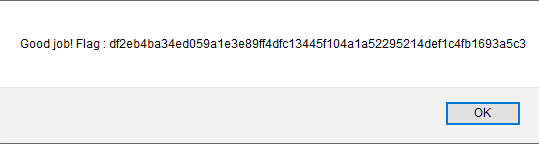
\includegraphics[width=0.5\textwidth]{07.Flag04/01-03.png}\\[0cm] 
\end{center}

It's possible for an attacker to steal and reuse
session identifiers or other sensitive cookie values
when they are stored or transmitted insecurely\cite{OWASPCookie}.

\subsection{Vulnerability}

\begin{figure}[!htb]
    \centering
    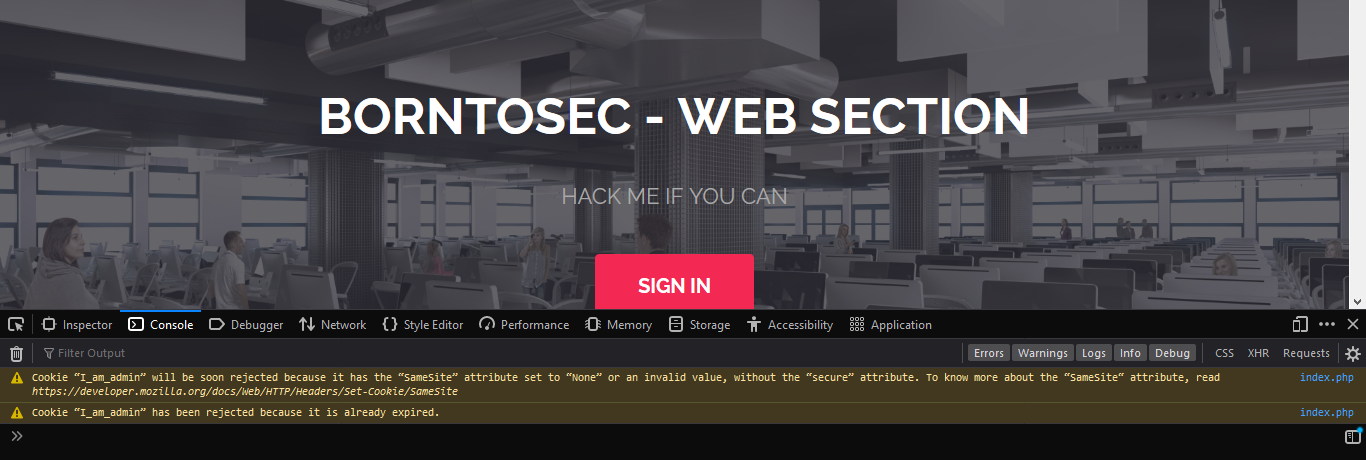
\includegraphics[width=0.752\textwidth]{07.Flag04/01-01.png}\\[0cm]  
    \caption[Cookie Alert]{Firefox refusing to set cookie `I\_am\_admin'}
    \label{fig:03-01 - Firefox rejects cookie iamadmin} 
\end{figure}
A cookie Vulnerability which is identified by OWASP as a
method to 'session-jack'\cite{OWASPCookie}.

\subsection{Location}

<ip-address>:80/index.php but also throughout the Web Application.

\subsection{Method}

I was immediately alerted by my console, for inspecting elements on
a webpage that there was something wrong with the cookie.

I proceeded to check the contents of the cookie and it was
an arbitrary string '68934a3e9455fa72420237eb05902327' (Figure \vref{fig: 3-2a cookie string}). The
cookie in question had:
\begin{itemize}
    \item[SameSite] - None
    \item[HttpOnly] - false
    \item[Secure] - false
\end{itemize}
It becomes clear what was to happen next which is determine if the string
has any meaning. After working out that the hash translated to 'false', I
decided to hash my own string equal to the string 'true'.
After refreshing the browser, the flag was returned.

The string 'true' = b326b5062b2f0e69046810717534cb09

\subsection{Tools}

\begin{figure}[!htb]
    \centering
    \subfloat[Console Screen showing cookie error]{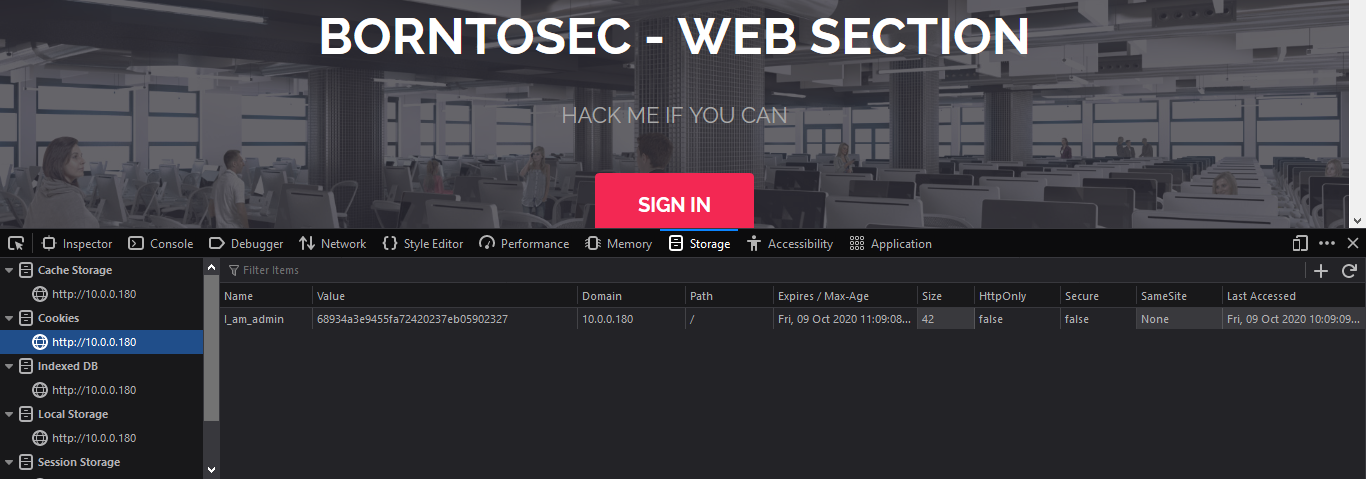
\includegraphics[width=.45\columnwidth]{07.Flag04/01-02a.png}\label{fig: 3-2a cookie string}} \quad
    \subfloat[Hash returning 'false']{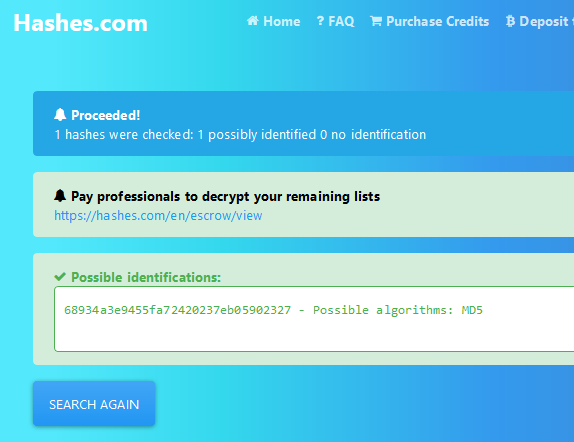
\includegraphics[width=.45\columnwidth]{07.Flag04/01-02b.png}\label{fig: cookie hash is false}} \\
    \subfloat[My own 'true' hash]{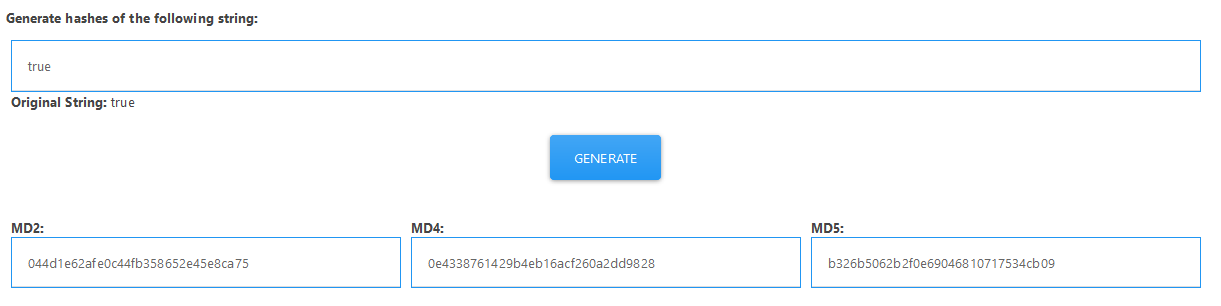
\includegraphics[width=.45\columnwidth]{07.Flag04/01-02c.png}\label{fig: 01 - My own true hash}} \quad
    \subfloat[Replaced hash \& ready to refresh]{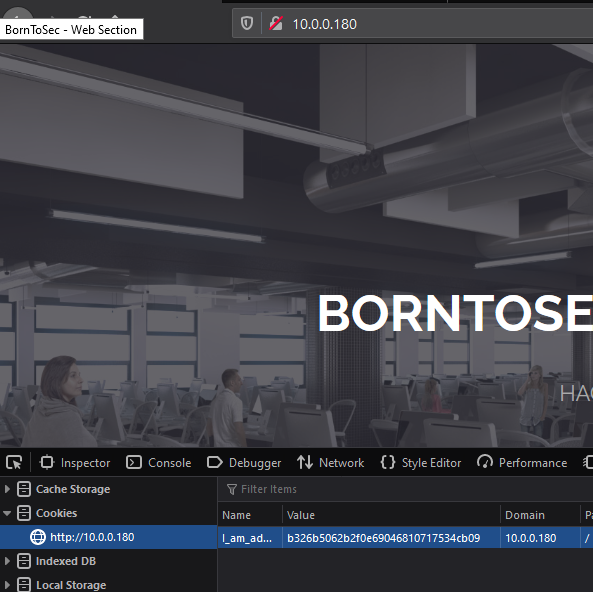
\includegraphics[width=.45\columnwidth]{07.Flag04/01-02d.png}\label{fig: 01 - Ready to refresh}}
    \caption[Flag 04 Method]{Process to Capture the Cookie Flag} % The text in the square bracket is the caption for the list of figures while the text in the curly brackets is the figure caption
    \label{fig:flag4 collection}
\end{figure}

The tools that I used were the console output of the 'Inspection Tool'
and the website \href{http://www.hashes.com}{hashes.com} in order to work
with the hashes.

\subsection{Remedy}

According to OWASP\cite{OWASPCookie} these are the steps one can take:
\begin{itemize}
    \item Make sure that all session identifiers are transmitted over an encrypted protocol.
    \item Terminate/regenerate the session if the session token is transmitted insecurely (either in clear text or as part of the URL), or signal to the application to do so.
    \item Enforce the Secure and HttpOnly flags on sensitive cookies using a Web Application Firewall.
    \item Ensure that session identifiers are transmitted only using the SSL session where they originated. Track sessions across SSL renegotiations and integrate with framework solutions to support common SSL termination/re-encryption architectures.
\end{itemize}